\section{Results}
We conducted a wide range of experiments during this study. The first experiments consisted of characterizing some commercial strips to get familiar with the the process and the equipment. Then, we conducted the same experiments with our custom strips. Lastly, we designed and tested our own potentiostat.

\subsection{Commercial strips}
The first step in this project was getting familiar with a commercial potentiostat and commercial electrodes. The glucose sensors were prepared in the manner described in the methodology. After manufacturing the sensors, we tested them with the BASi potentiostat using the amperometry mode with the initial potential at 700 mV, a sampling period of 120 seconds. The figure \ref{fig:basi} shows the results for three experiments conducted with three different glucose concentrations. These experiments show that the current changes when glucose was added to the solution and that the change is proportional to the concentration. This fact is summarized in figure \ref{fig:ci}.


\begin{figure}[h] 
\begin{center}
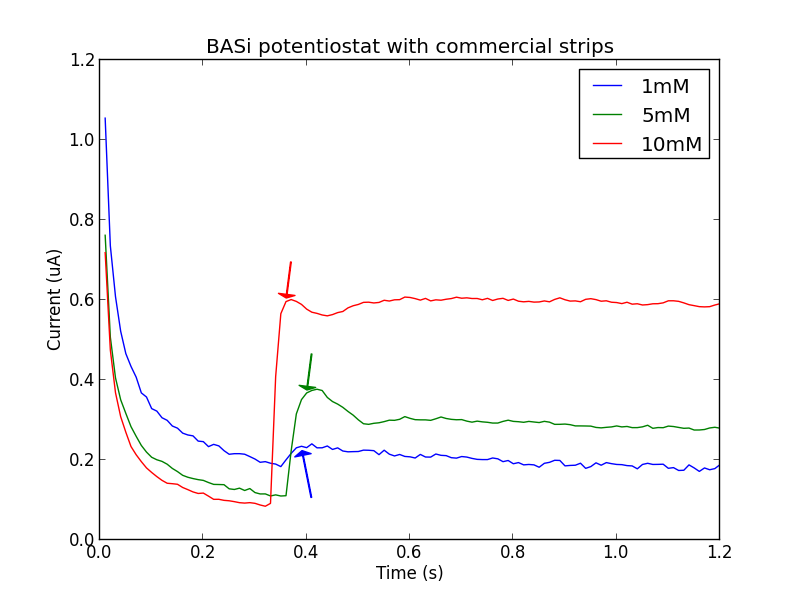
\includegraphics[width=3.5in]{../figures/basi.png}
\end{center}
\caption{Current vs. time plot for three different concentrations of glucose. These tests were done using a BASi potentiostat and commercial electrode strips. The arrow indicate responses to glucose being added to the solution.}
\label{fig:basi}
\end{figure}

\begin{figure}[h]
\begin{center}
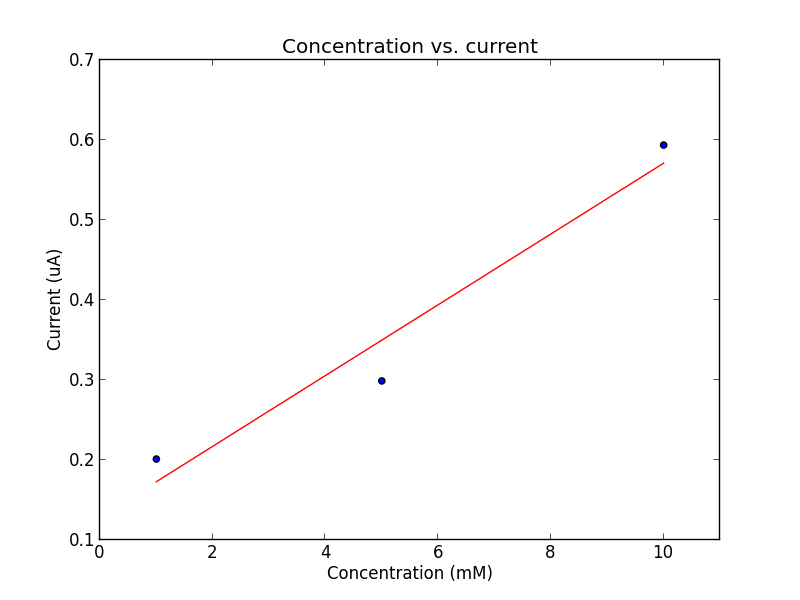
\includegraphics[width=3.5in]{../figures/CI.png}
\end{center}
\caption{Glucose concentration vs. current plot for three different concentrations of glucose. These tests were done using a BASi potentiostat and commercial electrode strips. Each data point is an average of currents after glucose was introduced.}
\label{fig:ci}
\end{figure}

\begin{figure}[h]
\begin{center}
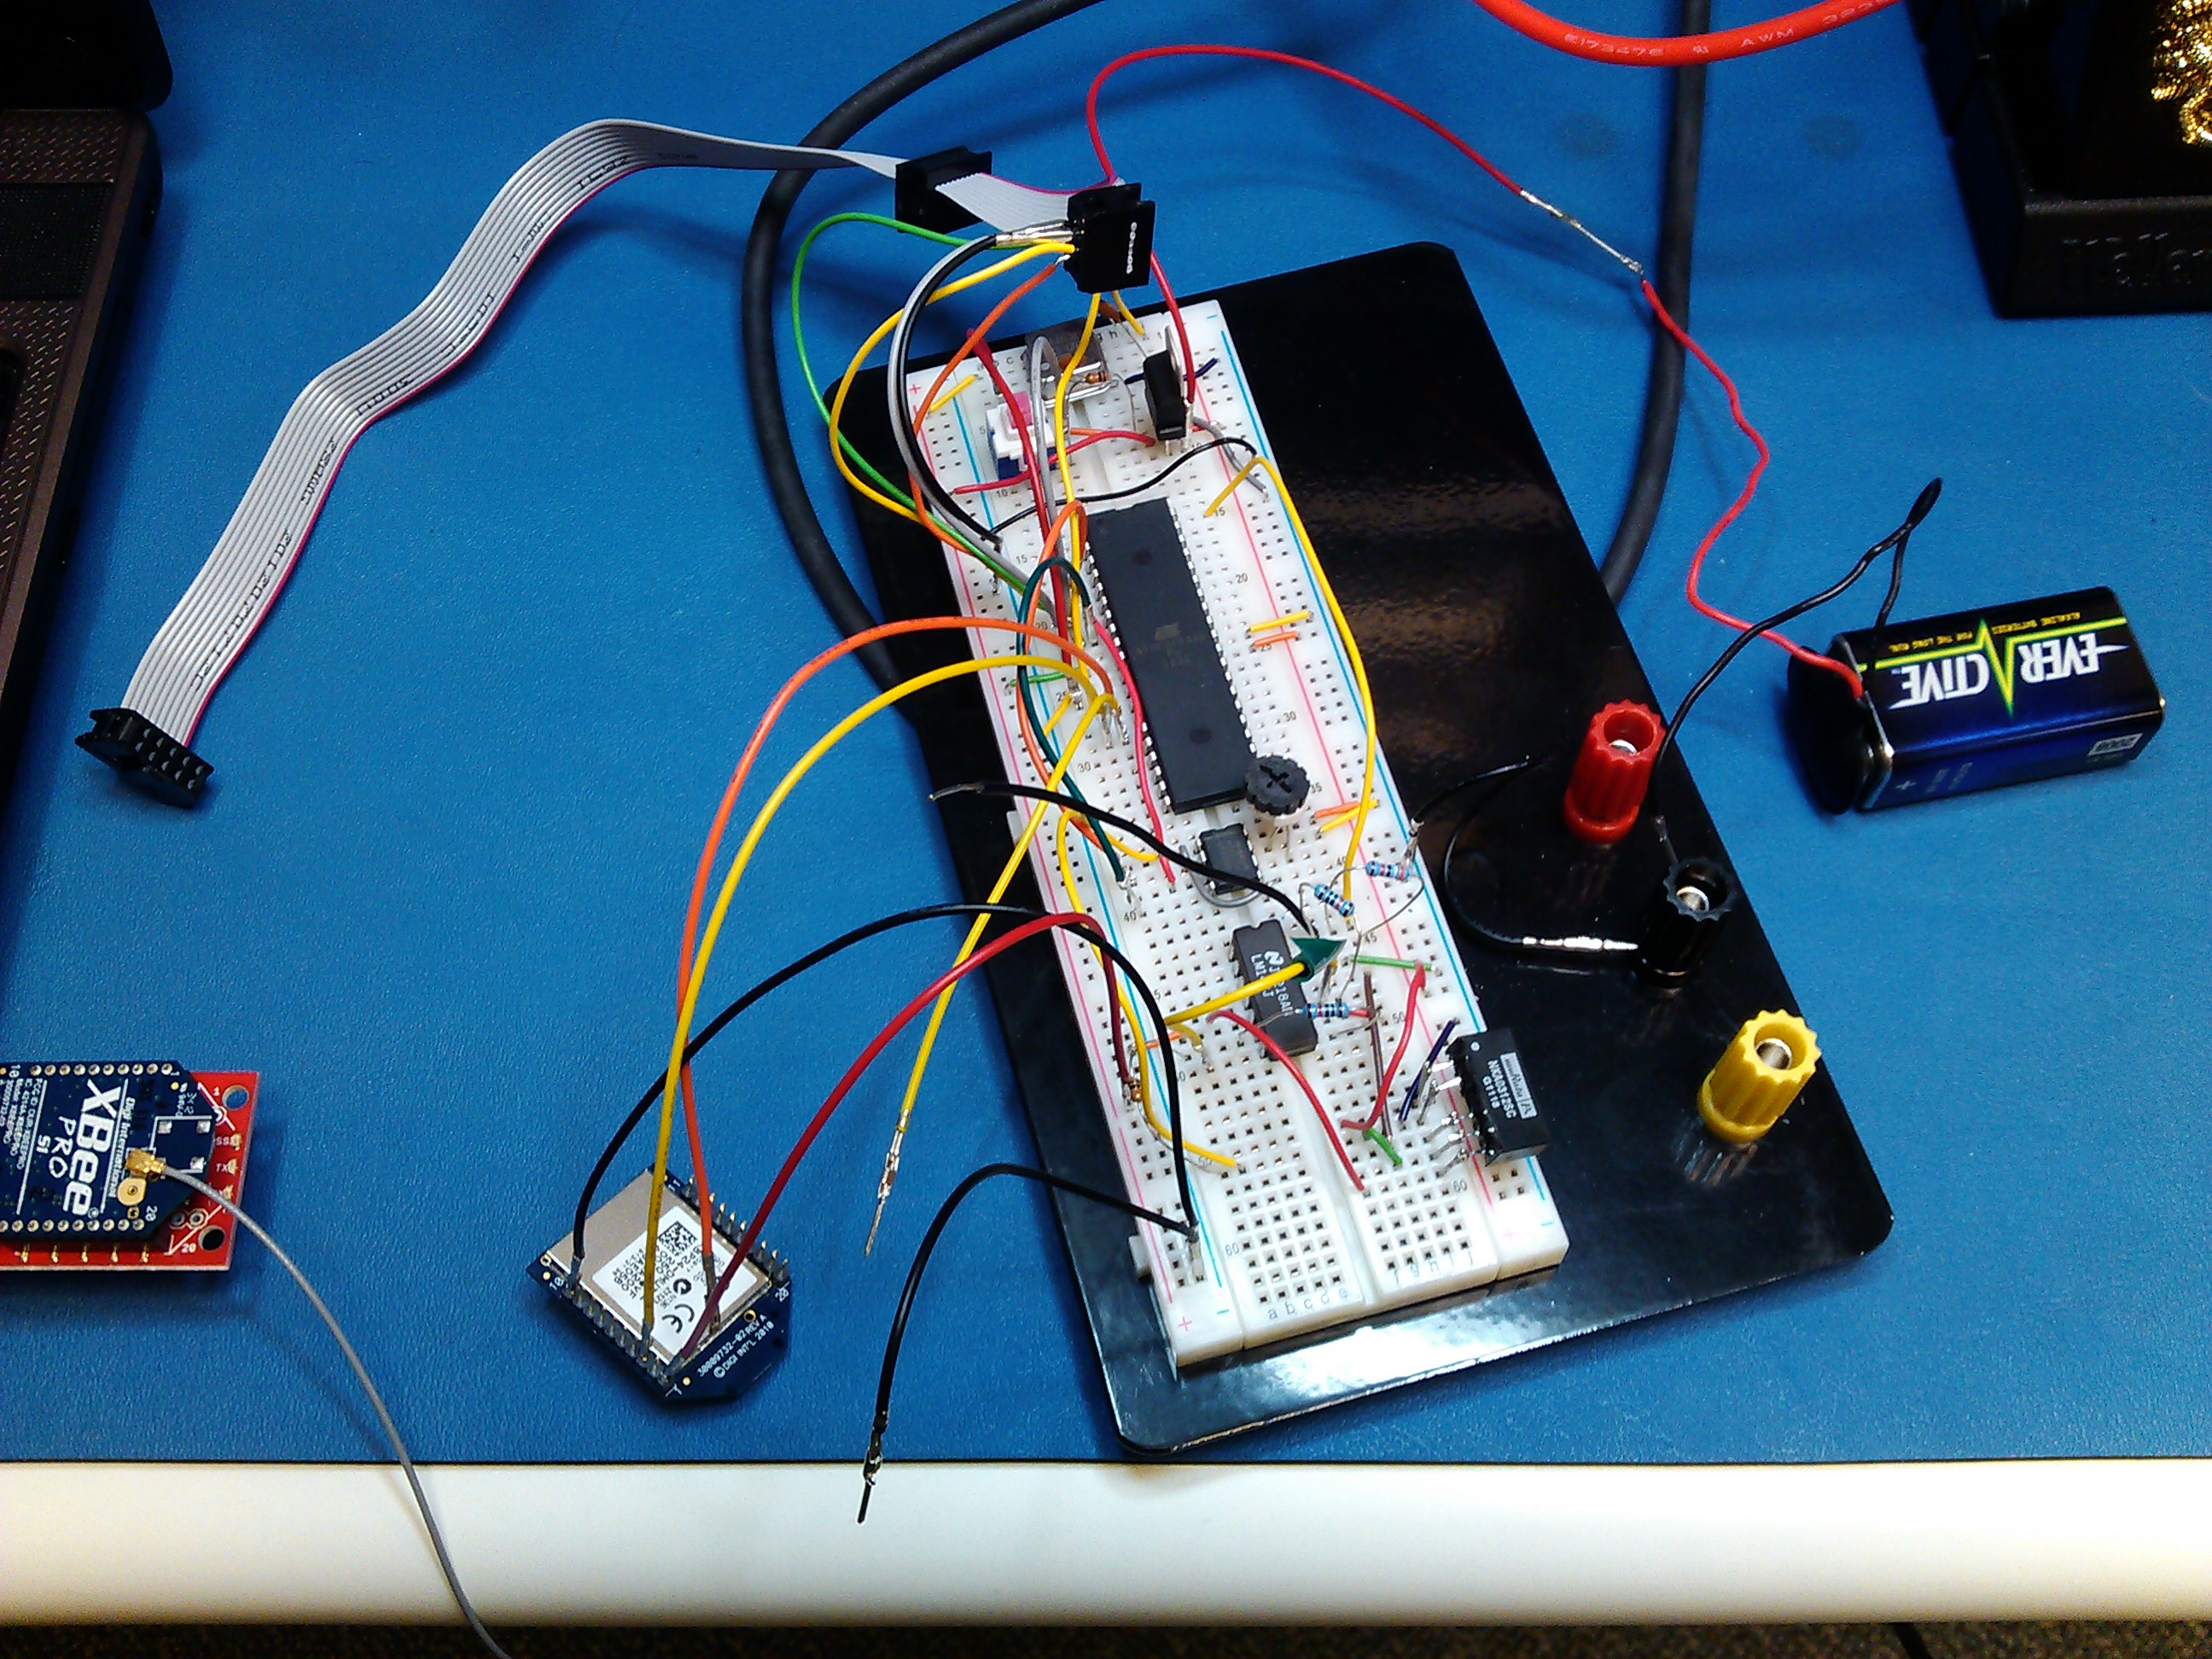
\includegraphics[width=3.5in]{../figures/board.jpg}
\end{center}
\caption{Picture of our system on a breadboard. The system can run off a 9V battery and communicates with a PC via XBee radio.}
\end{figure}

\subsection{Custom strips}
After collecting data with commercial strips, we proceeded to manufacture our own electrodes at TRC. We used the process described in the methodology and ended up with four electrodes. After manufacturing, we proceeded to immobilize the enzyme on the strips. We deviated from the procedure described in the methodology. The electrodes were not platinized or salinized before the functionalization process. When the receiving mixture was deposited on the active area it spread out of the active area all over the electrodes instead of staying in place. We deposited the receiving mixture on the commercial strips and the hydrogel stayed on the active area and did not spread. After all the strips were exposed to UV, each had gel on the active area and also had some visible glucose oxidase chunks that did not dissolve in the receiving mixture. 

Once the custom strips were ready, we tested them with the commercial potentiostat using the same settings as when we were testing the commercial ones. We were not getting any response. Even the commercial strips with the receiving mixture from the same batch were not giving us the proper response. After conducting multiple experiments, we decided to strip the wafers of the hydrogel and start over.

We stripped the hydrogel from the electrodes using isopropenol and salinized them. Then, we platinized all four electrodes at 700 mV for 60 seconds each and followed the rest of the procedure described in the methodology. After testing all the strips at various glucose concentrations, we did not see a response. Our best guess to why we were not getting correct results is that the isopropenol stripped the resist that was covering the wires and this created shorts which bypassed the active area. Due to these problems we were not able to characterize our sensors.
 
\subsection{Potentiostat implementation}
Designing the potentiostat involved looking at existing design, building the system, unit testing various functions of the system, and finally fine tunning and function testing the whole system.

\subsubsection{High level design}
The system consists of a  Atmega 644a microcontroller, running at 16 MHz, that is connected to a drive circuit and a measurement circuit. Data communication between the PC and the potentiostat is achieved through XBee radios operating in pass through mode. The drive circuitry is a 10 bit digital to analog converter (DAC) MAX5354 and an operational amplifier (opamp).  The schematic of the microcontroller based potentiostat is shown in the figure \ref{fig:pot_schem}. The list of components and the description is provided in figure \ref{fig:parts}.

\begin{figure} 
\begin{center}
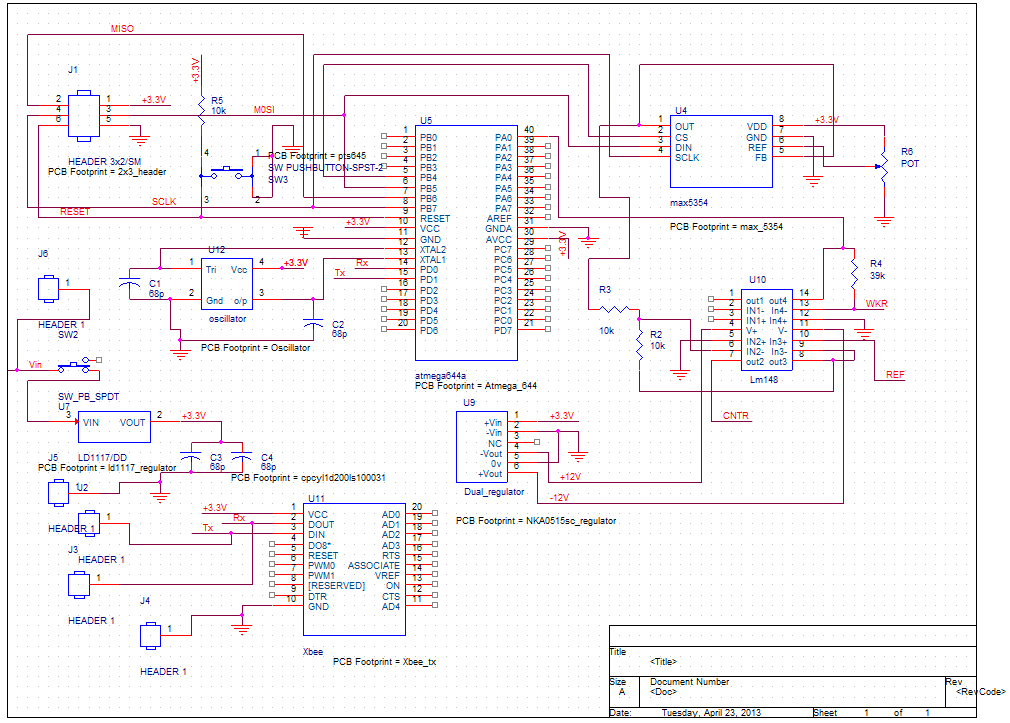
\includegraphics[width=3.5in]{../figures/potentiostat_schematic.png}
\end{center}
\caption{Schematic of potentiostat system design in Cadence Allegro.}
\label{fig:pot_schem}
\end{figure}


\begin{figure}
\begin{center}
\tiny
\begin{tabular}{l l l}
Part Reference & Part Number & Description \\
\hline
U4 & MAX5354 & 10 bit DAC \\
U5 & Atmega 644a &Microcontroller \\
U7 & LD1117 & 3.3 LDO voltage regulator \\
U9 & NKA0312SC & +/-12V dual voltage regulator \\
U10 & LM148 & Quad 4 Opam package \\
U11 & Xbee 802.15.4 & Xbee wire Antenna  \\
U12 & ECS-2200X & 16 Mhz crystal oscillator \\
c1,c2,c3,c4 & &68pf decoupling capacitors \\
R2,R3,R5 & & 10K biasing resistances \\
R4 & & 39K feedback resistance \\
R6 & & Pot to set reference voltage for DAC \\
SW3 & PVA1 EE H4  & Push Button switch DPST \\
SW2 & SPDT &  SPDT Mini Power Switch 
\end{tabular}
\normalsize
\end{center}
\caption{Parts list}
\label{fig:parts}
\end{figure}

\subsubsection{Drive and measurement circuit}
The drive and measurement circuitry consists of a DAC and an opamp circuit which is shown in \ref{fig:opamps}. The opamp circuit provides the constant voltage to the reference electrode (0.7 mV).   Input voltage to opamps A1 and A2 is set through the DAC. The input voltage is 1.2 V and through R1 and R2 it is converted to the 0.7 mV which is the input to the reference electrode. The current generated due to electrochemical reaction between the working and the reference electrode is converted to the equivalent voltage by the opamp A3 and the feedback resistor R3. The current between the working and counter electrodes is indirectly measured by the leftmost opamp. In our design the opamps' positive and negative rails are supplied from a +/- 12 V dual output voltage regulator. Its output voltage is proportional to the current on its negative input port. This voltage is fed to one of the analog pins on the microcontroller. It is converted to equivalent digital value by the microcontroller with the on-chip 10 bit analog to digital converter (ADC). This digital value is written to the UART and is transmitted by the XBee radio to a PC.


\begin{figure} 
\begin{center}
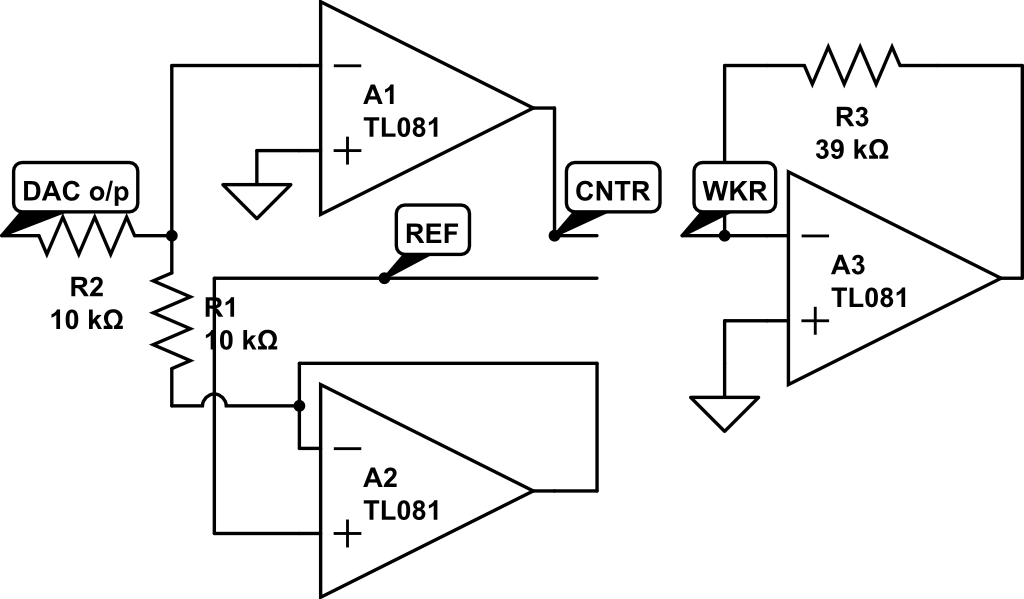
\includegraphics[width=3.5in]{../figures/opamps.png}
\end{center}
\caption{Opam circuits.}
\label{fig:opamps}
\end{figure}


\subsubsection{Sensitivity testing}
As shown in figure \ref{fig:sys_test}, we used resistance R4 instead of the glucose sensor to find the sensitivity and operating range of the potentiostat. To help fine tune the circuit, we used a simulator to find the optimal values for R4 and R3. In figure \ref{fig:sim} you can see the opamp circuit being simulated.

\begin{figure} 
\begin{center}
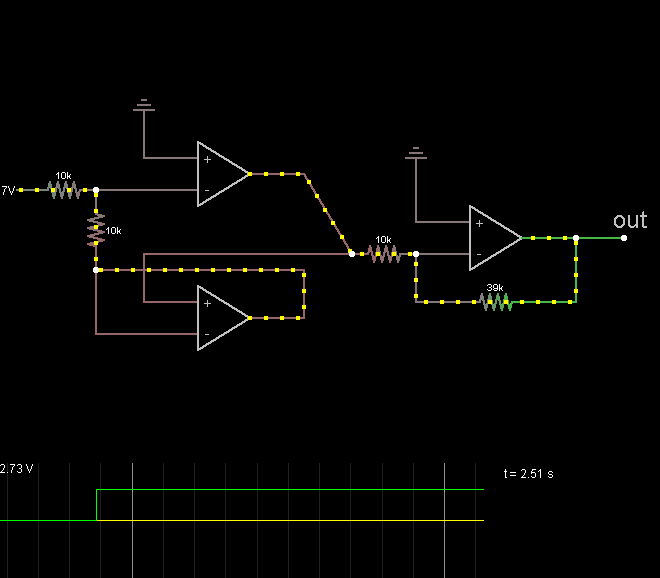
\includegraphics[width=3.5in]{../figures/circuit_simulator.png}
\end{center}
\caption{Simulation}
\label{fig:sim}
\end{figure}

Through simulation and experimentation we found the sensitivity of the potentiostat. Our potentiostat can measure the current in the range of 0.1uA to 70uA. Screen shots of low, mid and upper range tests can be seen in figures \ref{fig:sys_test_low}, \ref{fig:sys_test_mid}, and \ref{fig:sys_test_up}. The PC software  shown in the screen shot was developed in Python and uses pySerial for serial port communication and wxPython for the gui.

\begin{figure} 
\begin{center}
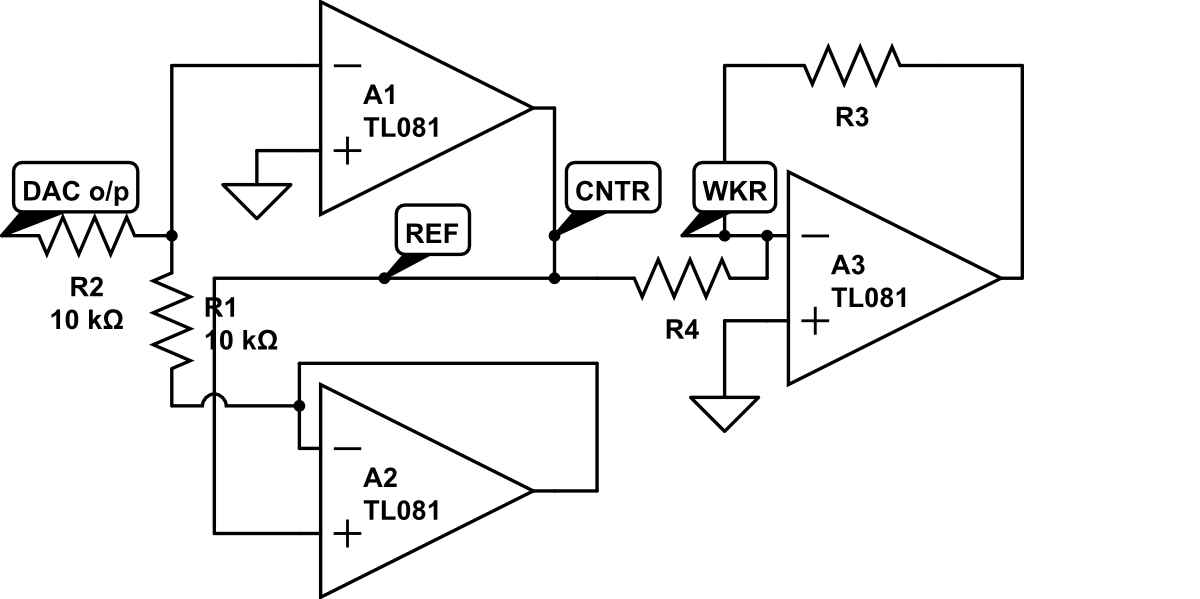
\includegraphics[width=3.5in]{../figures/system_testing.png}
\end{center}
\caption{System testing circuit.}
\label{fig:sys_test}
\end{figure}

%\small
\begin{center}
\begin{tabular}{l l l}
R4 & R3 & Current \\
\hline
10K$\Omega$ & 39K$\Omega$ & 70$\mu$A \\
1M$\Omega$ & 680K$\Omega$ & 8$\mu$A \\
6.8M$\Omega$ & 1M$\Omega$ & 0.1$\mu$A \\
\end{tabular}
\end{center}
%\normalsize

\begin{figure}[h]
\begin{center}
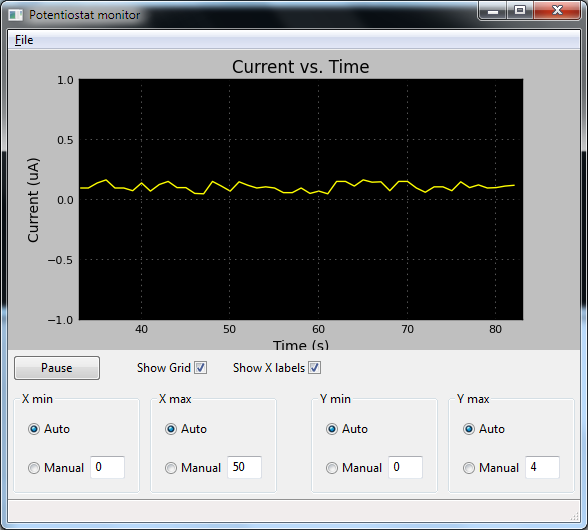
\includegraphics[width=3.5in]{../figures/1Mohm_0,1uA_6,8Mohm.png}
\end{center}
\caption{Low range}
\label{fig:sys_test_low}
\end{figure}

\begin{figure}[h]
\begin{center}
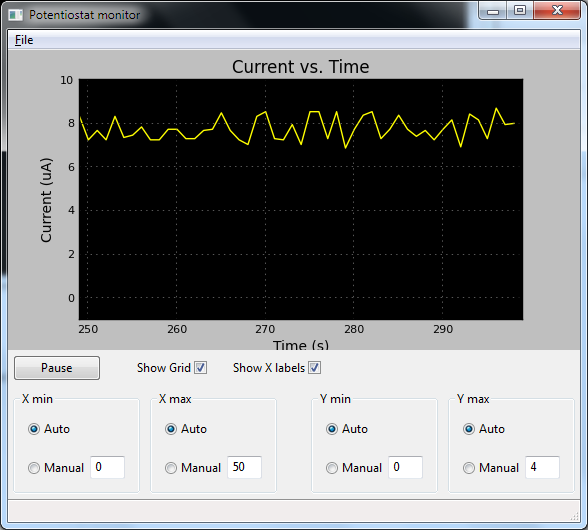
\includegraphics[width=3.5in]{../figures/1Mohm_8uA_680KOhm.png}
\end{center}
\caption{Mid range}
\label{fig:sys_test_mid}
\end{figure}

\begin{figure}[h]
\begin{center}
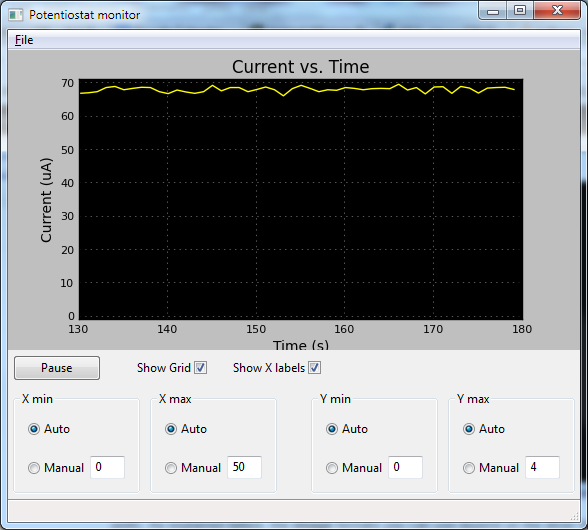
\includegraphics[width=3.5in]{../figures/10KOhm_70uA_39KOhm.png}
\end{center}
\caption{Upper range}
\label{fig:sys_test_up}
\end{figure}

\subsubsection{Board layout and power usage}
After breadboarding the system, using the Alegro PCB editor we designed a printed circuit board version of the system. We did not have time to fabricate the board. The system is fairly low power. Without the XBee radio, the system consumes 80 mA at 4.5 V and with the XBee radio 150 mA.

\begin{figure}[h]
\begin{center}
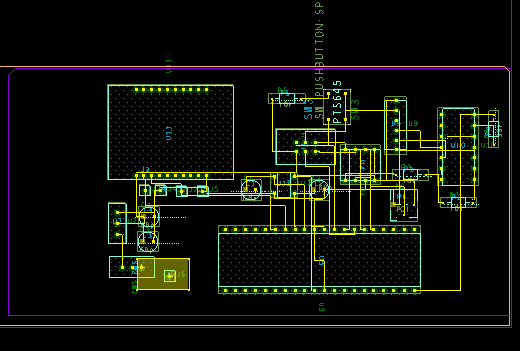
\includegraphics[width=3.5in]{../figures/layout.png}
\end{center}
\caption{Board layout}
\label{fig:sys_test_up}
\end{figure}